
\newcommand{\imagw}[3]{
  \begin{figure}[!hbt]
    \centering
    \includegraphics[width=#1]{#2}
    \caption{#3}
    \label{fig:#2}
  \end{figure}
}

\newcommand{\imag}[2]{\imagw{16cm}{#1}{#2}}

\chapter{A prototype for spatio-angular illumination}
\begin{summary}
  We give a general overview of the system, followed by more detailed
  explanation of some if its components. Then we introduce a model
  that allows to construct optimized masks for spatio-angular
  illumination.
\end{summary}

\nomenclature{MEMI}{Micro-mirror enhanced micro-imaging. EU FP7
  project reference 215597.}
\section{Overview}
\figref{fig:memi-simple} shows a simplified schematic of our optical
system. The uniform light distribution from the end of a light mixing
tunnel is imaged into the specimen. Two spatial light modulators allow
to modify the light intensity and angular distribution of the light
within the sample.

\begin{figure}[!hbt]
  \centering
  \def\svgscale{1.5}
  \input{memi-simple.eps_tex}
  \caption{Simplified schematic of the MEMI system. Light coming from
    the source is homogenized in an integrating tunnel. The light then
    traverses two spatial light modulators. The first of which (MMA)
    is imaged into the back focal plane of the objective and the
    second (LCoS) into the sample.}
  \label{fig:memi-simple}
\end{figure}

\figref{fig:hourglass-all} visualizes how our optical system improves
sample illumination. If the LCoS illuminates one in-focus
bead\footnote{Note that the LCoS acts as a Fourier filter on the
  information coming from the MMA. Therefor if all but a single pixel
  of the LCoS block the light, no angular control is possible (see
  also Appendix~\ref{sec:sim-angle}).}, the MMA can be used to prevent
exposure of the out of focus bead in
\figref{fig:hourglass-all}~(a). Not exciting the out-of-focus bead has
two advantages:
\begin{enumerate}
\item There is less background light in the camera image, leading to a
  clearer image of the in-focus information. It would be possible to
  computationally distinguish and subtract out-of-focus light by
  structured illumination methods but these methods will not remove
  the poisson distributed photon noise of the out-of-focus light.
\item Not exciting the out-of-focus areas is especially important for
  biological specimen in order to reduce the phototoxicity of the
  imaging.
\end{enumerate}
If an extended in-focus area should be imaged
(\figref{fig:hourglass-all}~(d)). Then multiple exposures, each with
different patterns on LCoS and MMA, can be combined into an image of
the in-focus information with minimal exposure of out-of-focus
fluorophores.

This technique requires prior knowledge about the fluorophore
distribution in the sample. In 3D time lapse imaging of developing
embryos a good estimate is available when the stacks are acquired with
high enough temporal resolution. Opto-genetics experiments can be
designed such, that the 3D distribution of neurons is known before
single neurons are triggered by light without exposing its neighbours.

\begin{figure}[!hbt]
  \centering
  \def\svgscale{.43}
  \input{hourglass-all.eps_tex}
  \caption{{\bf (a)} Two fluorescent beads are illuminated by all
    angles that an objective can deliver. The sharp image of the
    in-focus bead is deteriorated by blurry fluorescence of the out of
    focus bead. {\bf (b)} Angular control allows selective
    illumination of the in-focus bead and results in a better image on
    the camera. {\bf (c)} Angular control is insufficient, when an
    extended in focus area is illuminated. {\bf (d)} However,
    simultaneous spatial and angular control allows sequential
    excitation of the in-focus beads while excluding the out of focus
    bead.}
  \label{fig:hourglass-all}
\end{figure}
\newpage
\section{Detailed explanation of the optical components}

In the real system the spatial light modulators are reflective. 
Also both displays are not direct intensity modulators.
\figref{fig:memi-real} shows a schematic of the light path in
the combined angular and spatial control system.

A laser light source is scrambled by a rotating microlens array and
mixed in an integrating tunnel with a quadratic cross section.

The distance between the exit of the integration tunnel and the lens
$L_1$ is equal to the focal distance of $L_1$. The MMA is positioned
in the other focal plane of $L_1$. The micro mirror array consists of
$256\times 256$ mirrors with a pitch of \unit[16]{$\mu$m} (see
\figref{fig:mma} and \figref{fig:mma-closeup}). Each mirror hangs on
two thin hinges and can be tilted by up to $2^\circ$ by electrostatic
fields. CMOS circuits below each mirror allow to maintain a constant
tilt for hundreds of milliseconds. A dedicated control board can set
new analogue voltages with 10 bit resolution for each mirror in
\unit[850]{$\mu$s}. This enables framerates of up to \unit[1]{kHz} at
duty cycles up to \unit[50]{\%}.

When all mirrors of the MMA are flat, an image of the tunnel exit $F'''$
is formed in the plane of the aperture $B_1$. The size of the aperture
is chosen to transmit just this image. When mirrors of the MMA are
tilted, they will slightly deflect the light, so that it no longer
passes through the aperture $B_1$. $B_1$ acts as a Fourier filter (or
Schlieren optics).

If the mirrors of half of the device are deflected to fulfill the
blaze conditions\footnote{This is limited by the maximum tilt angle
  and possible for wavelengths up to \unit[800]{nm}} then the
corresponding area in the Fourier filtered image in $P'$ will be dark.

The lenses $L_2$ and $L_3$ relay the image of the tunnel exit $F'''$
from $F''$ into the plane $F'$ with the LCoS (ForthDD SXGA, pixel
pitch $\unit[13.62]{\mu m}$). The polarizing beam splitter ($45^\circ$
wire grid polarizing beam splitter, Moxtek) reflects linearly
polarized light towards the LCoS\footnote{In order to prevent spurious
  reflections at the PBS surface without wire grid and to improve
  contrast, the incoming light should already be polarized}. The
electric field vibrates perpendicular to the paper plane. Depending on
the LCoS pixel state (on or off) an LCoS pixel can rotate the
polarization of the returning light, so that it is
transmitted\footnote{As it is used in transmission a curvature of the
  PBS doesn't affect the quality of the LCoS image in the sample $F$
  as if the PBS was used in reflection.}  into the illumination tube
lens $\textrm{TL}_\textrm{ill}$ by the PBS (see \figref{fig:lcos} for
a photograph showing tube lens, PBS and LCoS).

The LCoS is ferroelectric (see \cite{1991Saleh} and \cite{Goodman1996}
p.~192).  Its liquid crystalls can swap very fast between two stable
orientations. In order to prevent a net current, which would
eventually destroy the device, its driver always displays an inverted
image after the wanted one. Therefor it is necessary to shutter the
light source accordingly.

The lenses $L_3$ and $\textrm{TL}_\textrm{ill}$ relay the Fourier
filtered MMA image from $P'$ into the pupil $P$ of the objective. In
order to accommodate objectives with various back focal plane
diameters, the illumination tube lens is built out of three lens
groups. Its focal length can be varied from \unit[222.8]{mm} up to
\unit[445.4]{mm} (see \figref{fig:memi-sketch} for a drawing with the
focal length of the other lenses). The lens groups move such, that the
image of the LCoS behind $\textrm{TL}_\textrm{ill}$ stays in infinity
and the the MMA (plane $P''$) is imaged into the pupil $P$, which is
\unit[250]{mm} behind behind the tubelens. \figref{fig:tubelens-bfp}
shows the pupil plane $P$ for two different settings of the focal
length of the tube lens.

Fluorescent light returns from the objective and is reflected by the
dichroitic beam splitter (DBS) through the detection tube lens
$\textrm{TL}_\textrm{det}$ and is imaged on the camera. Note that the
detection works with full efficiency.

\begin{figure}[!hbt]
  \centering
  \def\svgscale{2}
  \input{memi-real.eps_tex}
  \caption{Schematic of the light path through our microscope. Laser
    light enters from the lower left, is scrambled and homogenized to
    illuminate the full MMA and LCoS. $F$ is the field plane in the
    sample and its primed versions are conjugated planes. $P$ is the
    pupil of the objective. $B_0$ and $B_1$ are adjustable circular
    apertures. PBS is a polarizing beam splitter. DBS is a dichroitic
    beam splitter.}
  \label{fig:memi-real}
\end{figure}


\imagw{14cm}{setup-photo-blueprint}{The widefield epi-fluorescent
  microscope with attached illumination head. The positions of the two
  spatial light modulators (Micro mirror array (MMA) and liquid
  crystal on silicon display (LCoS)) are indicated. Drawing by Josef
  Wenisch (In-Vision, Austria).}

\imagw{14cm}{mma}{{\bf left:} Scanning electron microscope image of
  the micro-mirror array (MMA).  The pixel pitch of the device is
  \unit[0.016]{mm}. The hinges for the tilt movement and the
  electrodes are clearly visible. {\bf middle:} Optical reflective
  microscope image of the MMA. {\bf right:} exaggerated rendering of
  how a 8x8 checker board pattern would be displayed on the
  device. Electron and optical micrograph by Fraunhofer IPMS Dresden
  (Germany)}

\begin{figure}[!hbt]
  \centering
  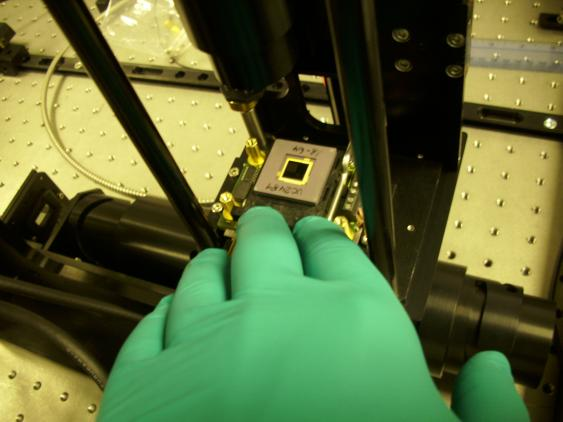
\includegraphics[width=7cm]{mma-plain}
  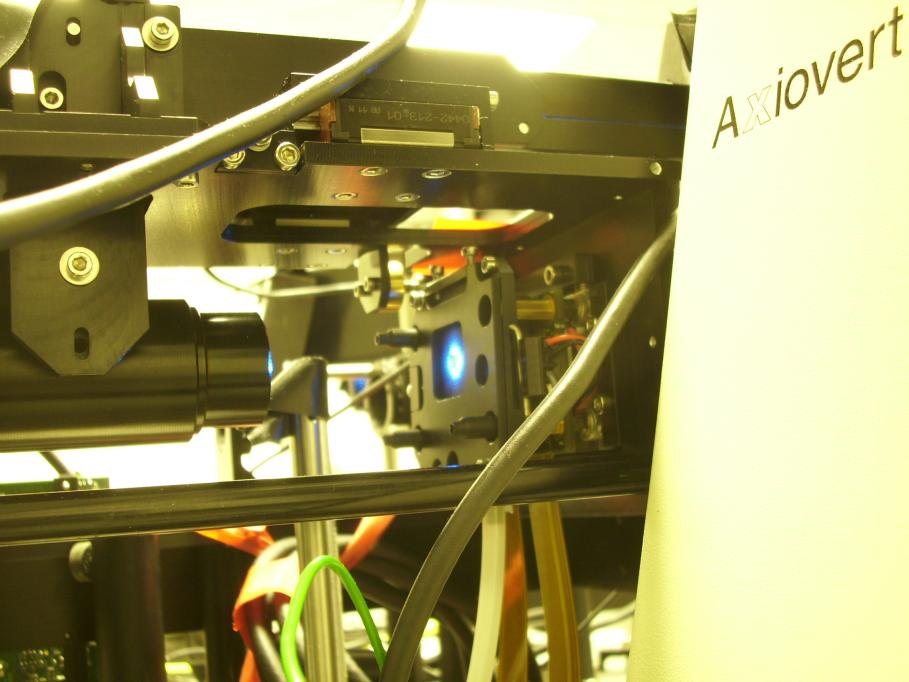
\includegraphics[width=7cm]{mma-ill}
  \caption{{\bf left:} Micro mirror array chip during installation of
    the optics. {\bf right:}~Illuminated micro mirror array in the
    aligned system.}
  \label{fig:mma-closeup}
\end{figure}

\begin{figure}[!hbt]
  \centering
  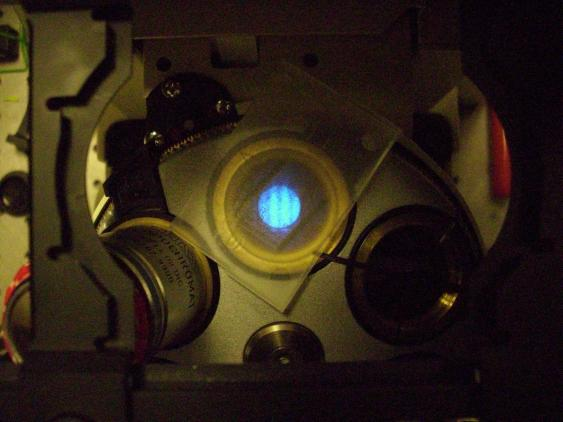
\includegraphics[width=7cm]{bfp1}
  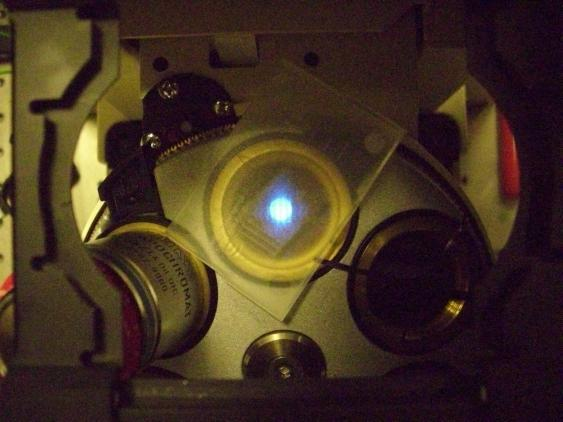
\includegraphics[width=7cm]{bfp2}
  \caption{Images of the micro mirror array in the back focal plane
    with different settings of the variable tubelens. The micro mirror
    array displays the same image (a disk) in both cases.}
  \label{fig:tubelens-bfp}
\end{figure}

\imagw{5cm}{lcos}{The black cylinder on the left is the variable tube
  lens. Behind this is the polarizing beam splitter and the
  ferroelectric liquid crystal on silicon display.}
\newpage
\section{Electronics for synchronization}
Both spatial light modulators can run at most with $50\%$ duty
cycle. Therefor it is necessary to synchronize the displays. Their
controllers allow to upload several hundred frames of image data
before an experiment and keep them in local storage. Images can then
be selected by fast function calls over USB (LCoS) or ethernet (MMA).

The camera (Andor Clara) as the slowest device is chosen as the
master. The camera provides two TTL outputs. The output ``fire'' is
high while the camera is integrating. The output ``shutter'' goes high
\unit[1]{ms} before ``fire'' and provides enough time
(\unit[$>850$]{$\mu$s}) for the MMA controller to tilt and let the
mirrors settle.

The LCoS controller can only be programmed to a limited number of
discrete image times (\unit[20]{ms}, \unit[10]{ms}, \unit[5]{ms},
\unit[200]{$\mu$s}) and it is not straight forward to change this via
USB interface. Therefor we always work with a fixed integration time
of \unit[20]{ms}. The ``fire'' output of the camera also switches the
laser on using an acousto optic modulator (AOM).

When the z-stage is used, the camera is stopped until the stage has
reached its target position.

\begin{figure}[!hbt]
  \centering
  \input{memi-electronics.eps_tex}
  \caption{The camera triggers both spatial light modulators with its
    TTL outputs. The acousto optic modulator sends light into the
    system during camera integration.}
  \label{fig:memi-electronics}
\end{figure}

\section{Alignment of the displays}

In order to be able to predict which position on the camera will be
illuminated by a particular pixel of the LCoS a calibration procedure
is run. For this a fluorescent plane is selected as a specimen. Then
single spots are scanned for a grid of $10\times10$ positions over the
LCoS. The resulting spots on the camera are located and four
parameters defining the rigid transform between camera and LCoS are
estimated (scale, rotation angle, translation in x and y, see
Appendix~\ref{sec:rigid}).

Using these parameters one can then convert between camera and LCoS
coordinates (see \figref{fig:screen_lcos-calib}). Changing the focal
length of the illumination tubelens or a change on the camera position
generally requires a new calibration.

\imagw{7cm}{screen_lcos-calib}{{\bf left:} Mask that is displayed on
  the LCoS. {\bf right:} Camera image of fluorescent plane illuminated
  by mask. The orange lines indicate the borders of the original
  pattern.}

The MMA is aligned by displaying an annular ring on the MMA and
matching it to the ring of a phase objective.


\section{Ray-based illumination optimization}
In order to make use of the spatio-angular illumination system it is
necessary to produce masks for the two spatial light modulators, that
will reduce unnecessary illumination in the sample.

\subsection{Index matched sphere model}
\label{sec:shadow-map}
One useful simple model is spheres. They can model fluorescent beads
or nuclei in a \emph{C.~elegans} embryo (see \figref{fig:render} for a
model constructed from confocal data). First we assume the beads are
embedded in index matched medium. Then rays only refract at the
gaussian sphere of the objective lens and it is insignificant how far
the target bead is from the interface between coverslip and medium
(see left drawing in \figref{fig:optimization_3}).

Suppose bead number zero should be excited but the out of focus beads
one to five should not be illuminated. One could then trace the cones
from the periphery of the out of focus beads through the target points
into the back focal plane of the objective. This gives a shadow map
and when one illuminates this particular target point using this mask
on the MMA, the out of focus beads are protected.

However, the last sentence isn't true for our system. If only one
pixel of the LCoS was enabled, hardly any information of the MMA mask
would reach the back focal plane. Instead the target area should be
increased, so that the LCoS doesn't act as a pinhole.

Then several shadow maps for different target locations (e.g.\ in a
region with \unit[3]{$\mu$m} diameter) can be combined and displayed
on the MMA.  Simultaneously the LCoS should display a mask that
selects the target region. In order to suppress ringing in the focal
plane it is helpful to display a smooth image on the MMA.

\imagw{8cm}{render}{Rendering of a sphere model, fitted to one time
  frame of a 3D confocal video of a developing \emph{C. elegans}
  embryo (strain AZ212, data provided by Jean-Yves Tinevez (Institut
  Pasteur, Paris) by finding local maxima in the difference of
  gaussian filtered data \citep{Santella2010}. The red rectangle would
  be selected for illumination with the LCoS. The red cylinder
  indicates the angle that would be least obscured by out of focus
  nuclei.}

\imagw{12cm}{scan-mosaic_testsample_n100_3_7_5_big}{}

\imagw{12cm}{scan-mosaic_nuc12_n100_3_7_5_big}{}



\imagw{12cm}{optimization_3}{Tracing rays from the periphery of out of
  focus spheres through an in-focus target point into the back focal
  plane of the objective results in a shadow map for the MMA.}



\subsection{Index mismatch}

Biological samples are often embedded in water. For spatio-angular
illumination the additional refraction at the glass--water interface
has to be taken into account.

The task of predicting where to mask the MMA in order to protect out
of focus beads is more complicated due to the spherical
aberrations. One would have to split the angular range and shift the
illumination spot on the LCoS correcing for the transversal focus
shift. For this one must have a good estimate of the distance of the
sample from the coverslip--water interface. See
Appendix~\ref{sec:raytrace} for a description of the raytrace
algorithm.

Another option is to use the HILO technique (see section
\ref{sec:hilo}) and generate a thin sheet of light with an MMA mask
that transmits close to the TIRF angle.


\begin{figure}[!hbt]
  \centering
  \def\svgscale{.3}
  \input{screen_0_lines.eps_tex} \quad \input{aberration-sketch.eps_tex}
  \caption{{\bf left:} Rays are starting from periphery of
    out-of-focus nucleus, hitting the target and refracted at the
    water--coverslip interface. {\bf right:} Due to spherical
    aberrations, rays from an on-axis point are shifted to $q(r)$ on
    the camera (where $r$ relates to the angle of the ray in the
    sample). }
\end{figure}
 
\begin{figure}[!hbt]
  \centering
  \bild{screen_microscope-aberrate}
  \caption{Raytracing through an objective followed by a tubelens. The
    focal length of the tubelens in this simulation is \unit[16]{mm}
    (as opposed to the usual \unit[160]{mm}) so that the plot fits
    into an unscaled image. The water depth is \unit[10]{$\mu$m}.}
  \label{fig:screen_microscope-aberrate-front}
\end{figure}

% our reports: they were often corrected by susan, so i should have a look
% MEMI_WP6_D6_5_Report.pdf     angular clem with grating on lcos
% 6.7    drawing of setup, alignment, sync image, only 11 of the 24 bitplanes
% 6.8a   full field angular control with mma (i used too large images on lcos)
%        rendering of c. elegans embryo, psf calc, ray model,
%        first (yellow) raytraces
% 8.6a   sync image with 11 out of 24
